\documentclass[conference]{IEEEtran}
\IEEEoverridecommandlockouts
% The preceding line is only needed to identify funding in the first footnote. If that is unneeded, please comment it out.
\usepackage{cite}
\usepackage{amsmath,amssymb,amsfonts}
\usepackage{algorithmic}
\usepackage{graphicx}
\usepackage{textcomp}
\usepackage{xcolor}
\usepackage{url} 
\def\BibTeX{{\rm B\kern-.05em{\sc i\kern-.025em b}\kern-.08em
    T\kern-.1667em\lower.7ex\hbox{E}\kern-.125emX}}
\begin{document}

\title{CS598 CCC Proposal\\
}

\author{
\IEEEauthorblockN{Cameron Greenwalt}
\IEEEauthorblockA{
\textit{UIUC}\\
Champaign, IL, USA \\
cg50@illinois.edu}
\and
\IEEEauthorblockN{Ming Meng}
\IEEEauthorblockA{
\textit{UIUC}\\
Champaign, IL, USA \\
mingm4@illinois.edu}
\and
\IEEEauthorblockN{Yang Peng}
\IEEEauthorblockA{
\textit{UIUC}\\
Champaign, IL, USA \\
yangp3@illinois.edu}
}
\maketitle


\section{Introduction and Project Idea}

AIOps, known as Artificial Intelligence for IT Operations, is a fairly recent development that focuses on applying machine learning to the IT Operations Space. AIOps is currently a hot area within the Cloud Computing Infrastructure. Many major technology corporations such as IBM and Microsoft \cite{li2022an}  are actively conducting research in the area of AIOps. \cite{aiops-challenges} 

One of the major concerns with AIOps in the industry is data privacy. Currently, when using proprietary/confidential data to train models, the data needs to be masked in some way to ensure security, which can require extensive time, preparation, and computational resources. Another big challenge in AIOps is that the cost and time required for training the models are often massive. We would like to use pre-trained Large Language Models (LLM) in the AIOps field and determine whether they can be used to remedy these challenges.

LLMs have seen tremendous recent breakthroughs, especially in the generative AI space. ChatGPT, which uses OpenAI's GPT 3.5 LLM, was publicly released in late 2022 and had immediate major impacts in many fields. Much research in the industry has been focused on applying LLM and generative chatbots such as ChatGPT to different domains. 

In this project, we aim to address data privacy concerns and avoid training an existing open source model \cite{network-log-anomaly-detection}  by 1) creating embedding vectors from the proprietary/confidential data source and 2) feeding those embedding vectors the latest state-of-art pre-trained LLM models available in the Azure Cloud.

Common AIOps tasks include, but are not limited to, log anomaly detection \cite{network-log-anomaly-detection}, node failure prediction \cite{aiops-node-failures-alibaba}, CI/CD of ML apps \cite{mlops-ossara}, test case generation and bug detection \cite{model-checking-guided-testing}, task code generation \cite{mani2023enhancing}, incident management \cite{chen2020aiops, li2022an}, and documentation Q\&A/source code understanding \cite{source-code-understanding}. We will apply the latest state-of-art LLM models in our proposed framework to at least one of these AIOps tasks and report our results.


\section{Justification}
In this section, we present the justifications of the project idea. We believe that this project fulfills all three areas of Intellectual Merit, Novelty, and impact.

\subsection{Intellectual Merit}
Currently, many researches in AIOps are done using models such as BERT \cite{network-log-anomaly-detection} and then further trained and finetuned using its own data. The results however are dismal \cite{network-log-anomaly-detection} in many categories due to issues such as proprietary data availability for training, open source model limitations, and limited GPU resources required to train the model. These challenges have hindered some of the development efforts in AIOps area.
In this project, we will create embedding vectors from proprietary data, use the embeddings as the datasource for finetuning an existing LLM (GPT 3.5) in Azure Cloud, and apply the fine-tuned model to at least one common AIOps task.
Since Azure Cloud is used by many big corporations, we believe that it should address the privacy concerns of proprietary data used for training a model.

For the above reasons, we believe that exploring common AIOps tasks using the latest state-of-art LLM should yield some interesting results.

\subsection{Novelty and Impact}
AIOps has been around for a while. However, as LLM is quite new and has only recently gained popularity due to the release of ChatGPT, most AIOps research still revolves around improving an existing model through further training or applying traditional ML and DL techniques \cite{network-log-anomaly-detection}. Improving an existing model can be a very expensive operation due to the amount of GPU required. Many businesses are unable to allocate the resources required to train a model from scratch. Using traditional ML and DL techniques requires expert domain and ML knowledge and often still requires expensive computation resources for training data.

By using pre-trained state-of-art models from existing Cloud Providers and providing the models with proprietary data, one can save computational resources and money by avoiding fine-tuning or training a model from scratch. This would be a more cost-effective way for businesses' IT teams to roll out AIOps solutions. This will in turn help the business' Site Reliability Engineers (SRE) to more effectively address cloud incidents.

If our experiments yield good results, we believe that our work will have a great impact to the AIOps field and that many non-tech companies can apply our methods in small teams of engineers to monitor and improve a company's complex cloud infrastructure environments.

\section{Preliminary plan}
We will start simple and then expand into more difficult tasks.
There are a few difficult areas identified for this project:
\begin{itemize}
    \item Dataset selection
    \item Creating embeddings and storing them in Vector stores
    \item Integration with Azure AI Services
    \item Usability
    \item Achieving Good Results
\end{itemize}
For data input, we will start with a simple pdf document, then try log data, technical documentations and specifications, cloud service configurations, and even source code (if time and intermediate results allow).
In order to make the service usable, we will identify scenarios that are common to current AIOps trends, which often includes incidents management and root cause analysis.

\subsection{What system do you want to implement?}\label{AA}
The system which we are going to implement is known as "A general AIOps framework using LLM-generated results". The system involves a user passing data to prompt generator and then entering a natural language query to the chatbot. The chatbot then generates a response by utilizing the query embeddings from the vector store.

\begin{figure}[ht]
    \centering
    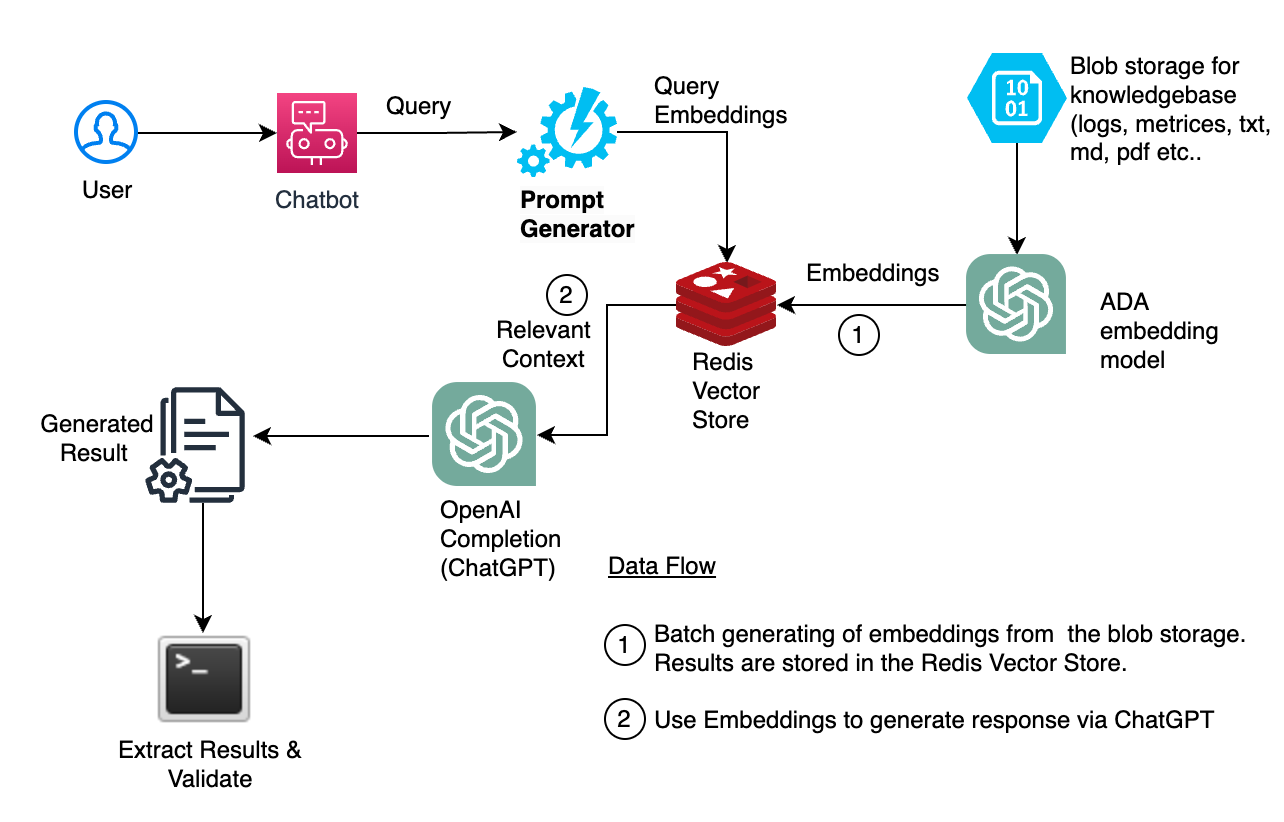
\includegraphics[width=0.5\textwidth]{arch.png}
    \caption{A proposed AIOps framework using LLM-generated results}
    \label{fig:arch}
\end{figure} 

Figure \ref{fig:arch} above shows the proposed implementation of the system. The chatbot can be either UI or API based. The vector store can be on Redis or the Azure's Cloud AI vector store. We will use Redis in our implementation. The ADA embedding model will convert the provided data source into vector embeddings, which will get stores in Redis. The chatbot then calls OpenAI ChatGPT model from Azure and generates the result. We will validate the generated result against a predefined text file for accuracy. 

There are a few key sections here for implementation: 
\begin{enumerate}
    \item Use of embedding model 
    \item Use of vector store 
    \item Output validation 
    \item Input data selection
    \item Methods of generating prompt responses using a LLM
\end{enumerate}

Each section has its own challenges and will significantly affect the result.


\subsection{What experiments do you think you'd need}
As stated we plan to start with something simple first to validate that the data flow works before performing a more complex task.

For the first experiment, we will select a simple pdf technical documentation of a cloud environment for our datasource to validate that the generated result of a simple prompt works fine. It could be a simple question such as "how-to" type of questions.

Then, we will start using AIOps tasks for our datasource. Data inputs for these tasks would probably include logs from different systems such as kubernetes, spark, cloud applications running on serverless environments, and network. This would be the main part of our experiment, in which we would measure the accuracy of the LLM on AIOps tasks.

We have read many research papers in regards to AIOps and those are detailed in the references section. We believe that we have a good grasp now on what type of logs we would like to experiment on and how the validation would work. 

Finally, if time permits, we could potentially extend this framework for further usages such as  to catch bugs for proprietary code, make design documents based on specifications and current proprietary architecture, and generate test cases for proprietary code. Whether we would want to proceed with this type of experiment or not will depend on whether we have time and the resources and whether our main goal of measuring AIOps is accomplished with good accuracy. 

\section{Summary}

Overall, we believe that our system is going to benefit companies of all sizes and improve their IT Operations workflows in a modern complex cloud infrastructure, as they often are unable to allocate the necessary resources and budget to train and finetune large ML models. We expect the following stakeholders to benefit from this project:
\begin{itemize}
    \item Site Reliability Engineers
    \item Platform Engineers 
    \item Management Audience 
    \item Incident Commanders 
\end{itemize}

We expect that SREs and Platform Engineers are the stakeholders that will benefit the most as our framework can used as an assistance tool for SREs when when performing Root Cause Analysis and can also be used to as a companion to the existing rule-based alerting tools \cite{model-checking-guided-testing}. Management Audience can use this tool to understand the current situation of the infrastructure without knowing many technical details. The incident commander can use this tool to ensure that the analysis is flowing in the right direction. Finally, we believe now is an optimal time to incorporate Generative AI into the corporate world within the IT Operations field. We hope this framework can transform how incident management, alerting, and root cause analysis are performed. 


\bibliographystyle{plain}
\bibliography{proposal}
\vspace{12pt}

\end{document}
\documentclass[conference]{IEEEtran}
\IEEEoverridecommandlockouts
% The preceding line is only needed to identify funding in the first footnote. If that is unneeded, please comment it out.
\usepackage{cite}
\usepackage{amsmath,amssymb,amsfonts}
\usepackage{algorithmic}
\usepackage{graphicx}
\usepackage{textcomp}
\usepackage{xcolor}
\usepackage{url} 
\def\BibTeX{{\rm B\kern-.05em{\sc i\kern-.025em b}\kern-.08em
    T\kern-.1667em\lower.7ex\hbox{E}\kern-.125emX}}
\begin{document}

\title{CS598 CCC Proposal\\
}

\author{
\IEEEauthorblockN{Cameron Greenwalt}
\IEEEauthorblockA{
\textit{UIUC}\\
Champaign, IL, USA \\
cg50@illinois.edu}
\and
\IEEEauthorblockN{Ming Meng}
\IEEEauthorblockA{
\textit{UIUC}\\
Champaign, IL, USA \\
mingm4@illinois.edu}
\and
\IEEEauthorblockN{Yang Peng}
\IEEEauthorblockA{
\textit{UIUC}\\
Champaign, IL, USA \\
yangp3@illinois.edu}
}
\maketitle


\section{Introduction and Project Idea}

AIOps, known as Artificial Intelligence for IT Operations, is a fairly recent development that focuses on applying machine learning to the IT Operations Space. AIOps is currently a hot area within the Cloud Computing Infrastructure. Many major technology corporations such as IBM and Microsoft \cite{li2022an}  are actively conducting research in the area of AIOps. \cite{aiops-challenges} 

One of the major concerns with AIOps in the industry is data privacy. Currently, when using proprietary/confidential data to train models, the data needs to be masked in some way to ensure security, which can require extensive time, preparation, and computational resources. Another big challenge in AIOps is that the cost and time required for training the models are often massive. We would like to use pre-trained Large Language Models (LLM) in the AIOps field and determine whether they can be used to remedy these challenges.

LLMs have seen tremendous recent breakthroughs, especially in the generative AI space. ChatGPT, which uses OpenAI's GPT 3.5 LLM, was publicly released in late 2022 and had immediate major impacts in many fields. Much research in the industry has been focused on applying LLM and generative chatbots such as ChatGPT to different domains. 

In this project, we aim to address data privacy concerns and avoid training an existing open source model \cite{network-log-anomaly-detection}  by 1) creating embedding vectors from the proprietary/confidential data source and 2) feeding those embedding vectors the latest state-of-art pre-trained LLM models available in the Azure Cloud.

Common AIOps tasks include, but are not limited to, log anomaly detection \cite{network-log-anomaly-detection}, node failure prediction \cite{aiops-node-failures-alibaba}, CI/CD of ML apps \cite{mlops-ossara}, test case generation and bug detection \cite{model-checking-guided-testing}, task code generation \cite{mani2023enhancing}, incident management \cite{chen2020aiops, li2022an}, and documentation Q\&A/source code understanding \cite{source-code-understanding}. We will apply the latest state-of-art LLM models in our proposed framework to at least one of these AIOps tasks and report our results.


\section{Justification}
In this section, we present the justifications of the project idea. We believe that this project fulfills all three areas of Intellectual Merit, Novelty, and impact.

\subsection{Intellectual Merit}
Currently, many researches in AIOps are done using models such as BERT \cite{network-log-anomaly-detection} and then further trained and finetuned using its own data. The results however are dismal \cite{network-log-anomaly-detection} in many categories due to issues such as proprietary data availability for training, open source model limitations, and limited GPU resources required to train the model. These challenges have hindered some of the development efforts in AIOps area.
In this project, we will create embedding vectors from proprietary data, use the embeddings as the datasource for finetuning an existing LLM (GPT 3.5) in Azure Cloud, and apply the fine-tuned model to at least one common AIOps task.
Since Azure Cloud is used by many big corporations, we believe that it should address the privacy concerns of proprietary data used for training a model.

For the above reasons, we believe that exploring common AIOps tasks using the latest state-of-art LLM should yield some interesting results.

\subsection{Novelty and Impact}
AIOps has been around for a while. However, as LLM is quite new and has only recently gained popularity due to the release of ChatGPT, most AIOps research still revolves around improving an existing model through further training or applying traditional ML and DL techniques \cite{network-log-anomaly-detection}. Improving an existing model can be a very expensive operation due to the amount of GPU required. Many businesses are unable to allocate the resources required to train a model from scratch. Using traditional ML and DL techniques requires expert domain and ML knowledge and often still requires expensive computation resources for training data.

By using pre-trained state-of-art models from existing Cloud Providers and providing the models with proprietary data, one can save computational resources and money by avoiding fine-tuning or training a model from scratch. This would be a more cost-effective way for businesses' IT teams to roll out AIOps solutions. This will in turn help the business' Site Reliability Engineers (SRE) to more effectively address cloud incidents.

If our experiments yield good results, we believe that our work will have a great impact to the AIOps field and that many non-tech companies can apply our methods in small teams of engineers to monitor and improve a company's complex cloud infrastructure environments.

\section{Preliminary plan}
We will start simple and then expand into more difficult tasks.
There are a few difficult areas identified for this project:
\begin{itemize}
    \item Dataset selection
    \item Creating embeddings and storing them in Vector stores
    \item Integration with Azure AI Services
    \item Usability
    \item Achieving Good Results
\end{itemize}
For data input, we will start with a simple pdf document, then try log data, technical documentations and specifications, cloud service configurations, and even source code (if time and intermediate results allow).
In order to make the service usable, we will identify scenarios that are common to current AIOps trends, which often includes incidents management and root cause analysis.

\subsection{What system do you want to implement?}\label{AA}
The system which we are going to implement is known as "A general AIOps framework using LLM-generated results". The system involves a user passing data to prompt generator and then entering a natural language query to the chatbot. The chatbot then generates a response by utilizing the query embeddings from the vector store.

\begin{figure}[ht]
    \centering
    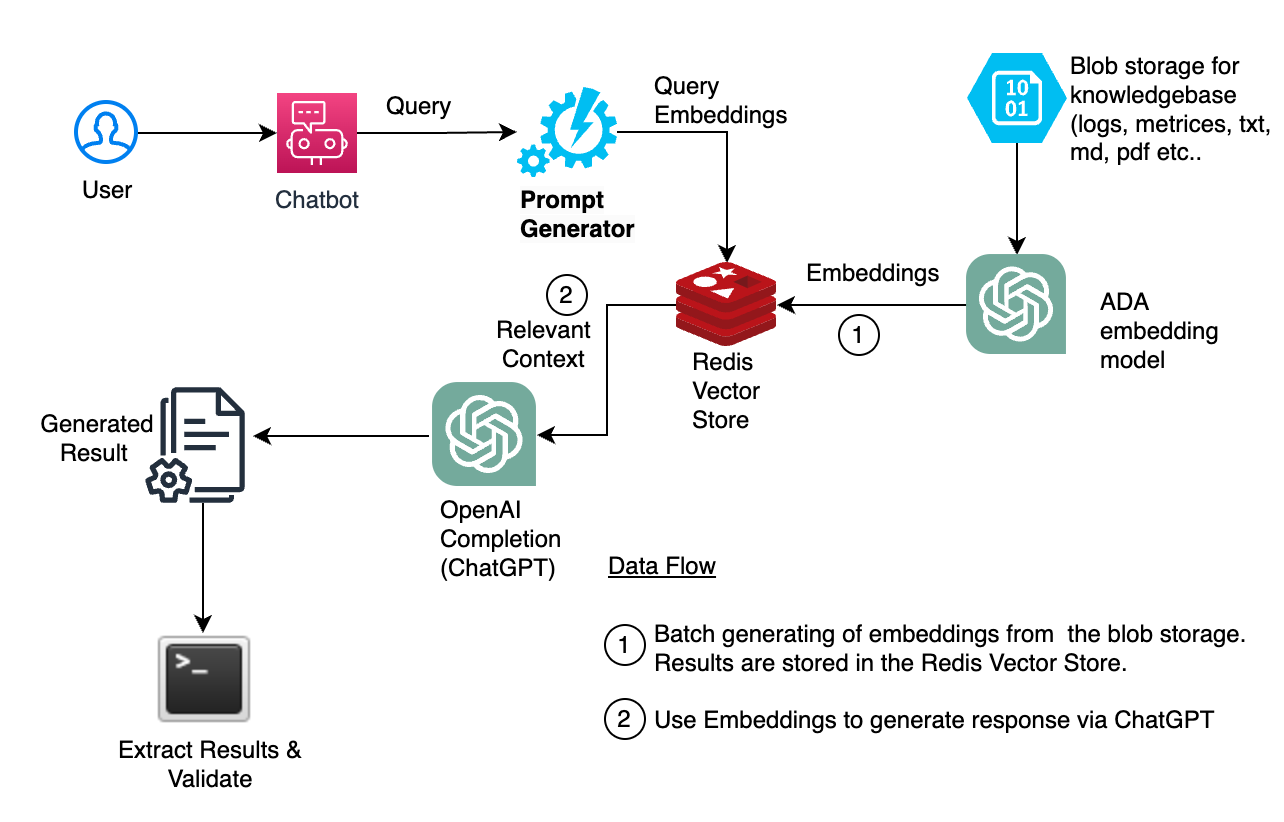
\includegraphics[width=0.5\textwidth]{arch.png}
    \caption{A proposed AIOps framework using LLM-generated results}
    \label{fig:arch}
\end{figure} 

Figure \ref{fig:arch} above shows the proposed implementation of the system. The chatbot can be either UI or API based. The vector store can be on Redis or the Azure's Cloud AI vector store. We will use Redis in our implementation. The ADA embedding model will convert the provided data source into vector embeddings, which will get stores in Redis. The chatbot then calls OpenAI ChatGPT model from Azure and generates the result. We will validate the generated result against a predefined text file for accuracy. 

There are a few key sections here for implementation: 
\begin{enumerate}
    \item Use of embedding model 
    \item Use of vector store 
    \item Output validation 
    \item Input data selection
    \item Methods of generating prompt responses using a LLM
\end{enumerate}

Each section has its own challenges and will significantly affect the result.


\subsection{What experiments do you think you'd need}
As stated we plan to start with something simple first to validate that the data flow works before performing a more complex task.

For the first experiment, we will select a simple pdf technical documentation of a cloud environment for our datasource to validate that the generated result of a simple prompt works fine. It could be a simple question such as "how-to" type of questions.

Then, we will start using AIOps tasks for our datasource. Data inputs for these tasks would probably include logs from different systems such as kubernetes, spark, cloud applications running on serverless environments, and network. This would be the main part of our experiment, in which we would measure the accuracy of the LLM on AIOps tasks.

We have read many research papers in regards to AIOps and those are detailed in the references section. We believe that we have a good grasp now on what type of logs we would like to experiment on and how the validation would work. 

Finally, if time permits, we could potentially extend this framework for further usages such as  to catch bugs for proprietary code, make design documents based on specifications and current proprietary architecture, and generate test cases for proprietary code. Whether we would want to proceed with this type of experiment or not will depend on whether we have time and the resources and whether our main goal of measuring AIOps is accomplished with good accuracy. 

\section{Summary}

Overall, we believe that our system is going to benefit companies of all sizes and improve their IT Operations workflows in a modern complex cloud infrastructure, as they often are unable to allocate the necessary resources and budget to train and finetune large ML models. We expect the following stakeholders to benefit from this project:
\begin{itemize}
    \item Site Reliability Engineers
    \item Platform Engineers 
    \item Management Audience 
    \item Incident Commanders 
\end{itemize}

We expect that SREs and Platform Engineers are the stakeholders that will benefit the most as our framework can used as an assistance tool for SREs when when performing Root Cause Analysis and can also be used to as a companion to the existing rule-based alerting tools \cite{model-checking-guided-testing}. Management Audience can use this tool to understand the current situation of the infrastructure without knowing many technical details. The incident commander can use this tool to ensure that the analysis is flowing in the right direction. Finally, we believe now is an optimal time to incorporate Generative AI into the corporate world within the IT Operations field. We hope this framework can transform how incident management, alerting, and root cause analysis are performed. 


\bibliographystyle{plain}
\bibliography{proposal}
\vspace{12pt}

\end{document}
